\documentclass[10pt,a4paper]{article}
\usepackage[utf8]{inputenc}
\usepackage{amsmath}
\usepackage{amsfonts}
\usepackage{amssymb}
\usepackage{listings}
\usepackage{graphicx}
\usepackage{caption}
\usepackage{subcaption}
\usepackage{float}
\lstset{showstringspaces=false,
		breaklines=true,
		postbreak=\raisebox{0ex}[0ex][0ex]{\ensuremath{\hookrightarrow\space}}}
    	
\begin{document}
\title{Intelligent Systems Assignment 4}
\author{Wessel Becker (1982362) \& Sander ten Hoor (2318555)}
\maketitle

\section{}
\subsection{}
\begin{figure}[H]
  \centering
    \makebox[\textwidth]{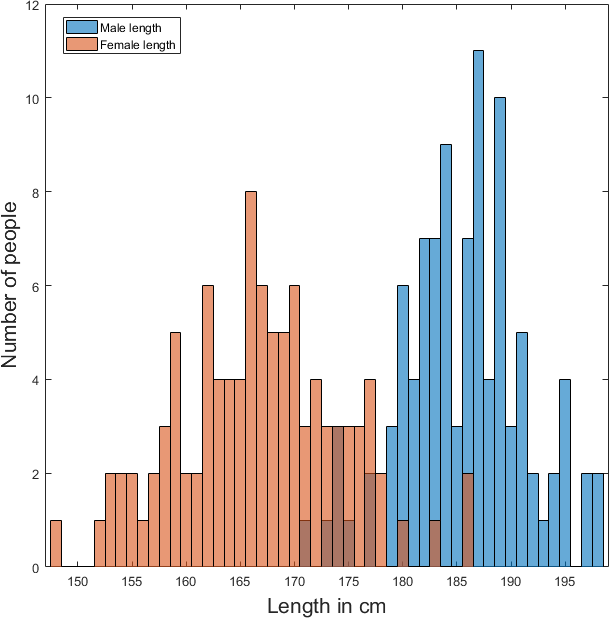
\includegraphics[width=\textwidth]{./images/1_1}} \\
  \caption{Histogram of height}
  \label{fig:1_1}
\end{figure}

\subsection{}
If the decision criteria is 170 cm with the assumption that everyone larger than 170 cm is male, there would be no men classified incorrectly. However, several women would be. Counting the bars representing women right of 170 cm gives us 29 incorrectly classified women.
(If 170 cm counts as men already, it is 29 + 6 = 35)

\subsection{}
If the decision criteria would be 178 cm, with everyone larger than 178 cm being male, the least number of classification errors would occur according to these histograms. It results in 8 classification errors for women and 4 for men.

\section{}
\subsection{}
\begin{figure}[H]
  \centering
    \makebox[\textwidth]{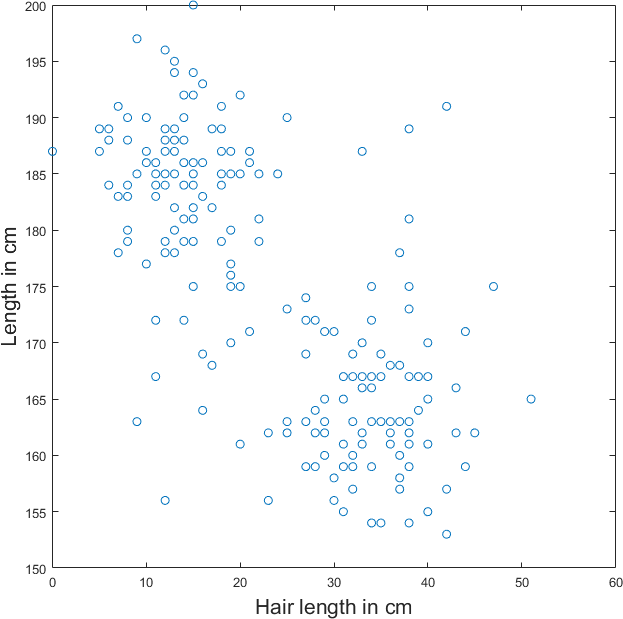
\includegraphics[width=\textwidth]{./images/2_1}} \\
  \caption{Histogram of height}
  \label{fig:1_1}
\end{figure}

\section{Matlab Code}

\section{Work done}

\end{document}